L'electrònica rep i processa el senyal elèctric emés pel fotosensor i emmagatzema la informació pertinent. Les diferents tasques executades per l'electrònica són aplicar llindars d'energia sobre el senyal (utilitzats per descartar senyals no pertanyents a esdeveniments de triti), amplificar el senyal (per tindre millor precisió en les operacions realitzades sobre aquest) i aplicar coincidències (per reduir el nombre d'esdeveniments no pertanyents al triti). Finalment es realitza un histograma dels senyals que han superat totes les etapes anteriors, obtenint un espectre d'energia. L'electrònica depén del tipus de senyal que reba i, per tant, del tipus de fotosensor emprat. A causa d'això, en la col·laboració TRITIUM s'utilitzen electròniques diferents, una per a les matrius de SiPMs i altra per als PMTs:

\begin{enumerate}

\item{} L'electrònica emprada per a quan s'utilitzen matrius de SiPMs s'anomena PETsys \cite{PETSYS}, mostrada a la Figura \ref{fig:PETSYSs}, un sistema comercial desenvolupat específicament per a treballar amb matrius de SiPMs. 

\begin{figure}[h]
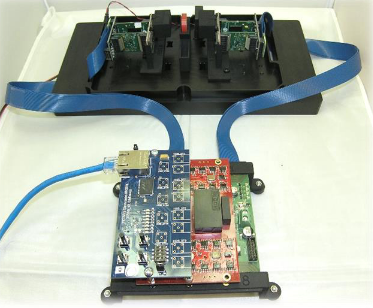
\includegraphics[scale=0.5]{12Summary/3DesignPrinciples/32Tritium_detector/PETSYS_System.png}
\centering
\caption{Sistema comercial PETsys\label{fig:PETSYSs}.}
\end{figure}

\item{} L'electrònica emprada quan s'utilitzen PMTs en assajos a l'interior de laboratoris es basa en tecnologia NIM, la qual és un tipus de tecnologia modular. L'equip portugués de la col·laboració TRITIUM va dissenyar i construir una electrònica específica que està basada en diverses targetes de circuit imprés (PCB per les sigles en anglés) les quals són utilitzades en Arrocampo, l'emplaçament final del detector.

\end{enumerate}